\chapter{Módulo \textit{Speech to Text} para \textit{Godot}}
\label{cap:stt-module}

Após adquirirmos conhecimento sobre a biblioteca \textit{Pocketsphinx} e a \textit{game engine} \textit{Godot}, chegou o momento de construirmos o módulo de reconhecimento de voz.

Conforme descrito na seção \ref{godotLanguages}, a linguagem \mbox{\textit{GDScript}} é extremamente prática para programar estruturas em um jogo feito em \textit{Godot}. No entanto, às vezes deseja-se otimizar alguma parte crítica através de \textit{C++} ou adicionar uma nova funcionalidade inexistente em \textit{Godot}. Os módulos servem justamente para este objetivo, pois não fazem parte do código essencial da \textit{game engine}.

Este capítulo documenta os passos e decisões de projeto tomados na criação do módulo, a qual chamaremos de \textit{Speech to Text}. Pressupomos que o leitor esteja familiarizado com as instruções para compilação de \textit{Godot}, vistas na seção \ref{godotCompile}, e com a biblioteca \textit{Pocketsphinx} (capítulo \ref{cap:pocketsphinx}), que será usada para a realização do reconhecimento de voz.

As instruções para criação do módulo foram baseadas no tutorial existente na documentação de \textit{Godot} \citep{godotModuleCreation}.

Todas as instruções e comandos apresentados foram originalmente realizados no sistema \texttt{Ubuntu 16.04 LTS, 64-bit} do autor.

% ---------------------------------------------------------------------

\section{Primeiros passos}

Antes de começarmos a implementar o módulo em si, precisaremos tomar algumas medidas simples de preparação.

\subsection{Criação do diretório do módulo}

Todos os módulos ativos são encontrados como subdiretórios dentro da pasta \texttt{modules/} no código fonte. Começaremos, portanto, com a criação do diretório \texttt{speech\_to\_text}:

\begin{lstlisting}[language=Bash]
$ cd modules
$ mkdir speech_to_text
$ cd speech_to_text
\end{lstlisting}

% ---------------------------------------------------------------------

\subsection{Adição do pacote \textit{Sphinxbase}}

Usaremos a biblioteca \textit{Pocketsphinx} para realizar o reconhecimento de voz no módulo. Um dos requisitos necessários para seu funcionamento, conforme visto na seção \ref{sphinxCompile}, é o pacote \textit{Sphinxbase}. A seguir, apresentamos instruções para inserir os arquivos essenciais deste pacote no diretório do módulo.

\begin{enumerate}
\item Baixe o pacote \textit{Sphinxbase} em sua versão atual mais estável, a \textbf{5-prealpha}.

\begin{lstlisting}
$ SPHINXURL="https://sourceforge.net/projects/cmusphinx/files"
$ wget $SPHINXURL/sphinxbase/5prealpha/sphinxbase-5prealpha.tar.gz
\end{lstlisting}

\item Extraia e renomeie o pacote baixado.

\begin{lstlisting}
$ tar -xvf sphinxbase-5prealpha
$ mv sphinxbase-5prealpha sphinxbase
\end{lstlisting}

\item Remova arquivos supérfluos, como \texttt{Makefiles}, arquivos de teste e \textit{scripts} de compilação. Estes serviriam para aumentar, desnecessariamente, o tamanho do módulo. Em outras palavras, somente as interfaces e implementações nos pacotes serão mantidas. Veja a listagem \ref{sphinxbaseEssential} para maiores detalhes.

\lstinputlisting[
  language=Bash,
  caption={Remoção de arquivos supérfluos no pacote \textit{Sphinxbase}},
  label={sphinxbaseEssential}]
  {listing/sphinxbase-essential.sh}
\end{enumerate}

% ---------------------------------------------------------------------

\subsection{Adição do pacote \textit{Pocketsphinx}}

Precisamos, também, do pacote \textit{Pocketsphinx} para a biblioteca homônima funcionar. A seguir, apresentamos instruções para inserir os arquivos essenciais deste pacote no diretório do módulo.

\begin{enumerate}
\item Baixe o pacote \textit{Pocketsphinx} em sua versão atual mais estável, a \textbf{5-prealpha}.

\begin{lstlisting}
$ SPHINXURL="https://sourceforge.net/projects/cmusphinx/files"
$ wget $SPHINXURL/pocketsphinx/5prealpha/pocketsphinx-5prealpha.tar.gz
\end{lstlisting}

\item Extraia e renomeie o pacote baixado.

\begin{lstlisting}
$ tar -xvf pocketsphinx-5prealpha
$ mv pocketsphinx-5prealpha pocketsphinx
\end{lstlisting}

\item Remova arquivos supérfluos, isto é, que não sejam interfaces ou implementações. Veja a listagem \ref{pocketsphinxEssential} para maiores detalhes.

\lstinputlisting[
  language=Bash,
  caption={Remoção de arquivos supérfluos no pacote \textit{Pocketsphinx}},
  label={pocketsphinxEssential}]
  {listing/pocketsphinx-essential.sh}
\end{enumerate}

% ---------------------------------------------------------------------

\section{Planejamento}

Quais os requisitos funcionais e não funcionais que queremos atender? O que um típico usuário do módulo \textit{Speech to Text} desejaria para poder usar em seu jogo? Todo projeto deve começar com algum planejamento mínimo de onde se quer chegar para obter algum sucesso.

% ---------------------------------------------------------------------

\subsection{Requisitos não funcionais}

% TODO: Fix references

Reconhecimento de voz em jogos geralmente é usado em um contexto de tempo real. Isto é, para uma dada fala do usuário, não desejamos que o jogo demore muito para dar alguma forma de resposta com o risco de comprometer seu aspecto lúdico. A preocupação é reduzida ao lembrarmos que \textit{Pocketsphinx} apresentou resultados rápidos nos testes realizados na seção \ref{???}.

Portanto, em termos dos principais parâmetros de reconhecimento de voz definidos na seção \ref{sttMainTerms}, projetaremos o módulo com a questão de \textbf{eficiência} em mente:

\begin{itemize}
\item \textbf{Fluência}: Idealmente, a forma de comunicação poderia chegar até \emph{palavras conectadas}. Uma \textit{fala contínua} demandaria um processamento muito pesado e comprometedor para o jogo.

\item \textbf{Dependência do usuário}: Um sistema \emph{independente} é mais flexível por atender a uma maior quantidade de pessoas sem a necessidade de um longo treinamento antes de começaram a jogar.

\item \textbf{Vocabulário}: Deve ser tipicamente \emph{pequeno} (não mais do que 40 palavras). Um vocabulário muito grande aumentaria a velocidade de reconhecimento, que por sua vez afetaria a experiência do jogador.

\item \textbf{Parâmetros ambientais}: Não é esperado que interfiram tanto no jogo. A relação sinal/ruído deve ser baixa, pois um ambiente muito barulhento comprometeria a jogabilidade. Por fim, desejamos que o usuário possa falar em um tom de voz normal, sem precisar ``forçar'' a pronúncia das palavras ou aumentar sem tom para o reconhecimento ser possível. Tais características são automaticamente tratadas pelo modelo acústico usado no \textit{Pocketsphinx}.
\end{itemize}

Desejamos que o módulo seja \textbf{confiável} em relação à acurácia do reconhecimento de voz. Conforme vimos na seção \ref{???}, isto dependerá dos modelos usados na configuração do \textit{Pocketsphinx}.

\textbf{Configurabilidade} também é uma característica desejada: o usuário do módulo deverá ter controle sobre a língua do reconhecimento e o vocabulário reconhecido, por exemplo. \textit{Pocketsphinx} permite isso facilmente com a alteração de seus arquivos de configuração, incluindo o modelo acústico e as palavras-chave.

O módulo deverá ser de \textbf{propósito geral} em relação ao tipo de jogo em que é empregado (ação, terror, plataforma, etc.); portanto, não é possível prever características do típico usuário do jogo. Este requisito, em geral, não é tão preocupante quando levamos em conta o uso de um modelo acústico geral com a biblioteca \textit{Pocketsphinx}.

É importante que o módulo seja \textbf{tolerante a erros}, isto é, que comunique ao restante do sistema quando um problema ocorre dentro de si.

Por fim, um requisito desejável, mas a princípio não estritamente necessário, é a  \textbf{portabilidade}. Apesar das classes internas de \textit{Godot} e a biblioteca \textit{Pocketsphinx} terem sido projetados para funcionarem em diversos sistemas operacionais, colocaremos plataformas \textit{Unix} como a meta principal. Suporte a outras plataformas poderá ser feito depois, dependendo da complexidade da implementação.

% ---------------------------------------------------------------------

\subsection{Requisitos funcionais}
\label{moduleFunctionalRequirements}

A princípio, desejamos que o reconhecimento de voz seja executado em paralelo com o restante do jogo. Isto é, gostaríamos que a execução não parasse totalmente até obter um comando por voz do usuário. Queremos, também, uma forma de verificar se o reconhecimento está ativo e de iniciá-lo/desligá-lo a qualquer momento.

As palavras reconhecidas pelo módulo \textit{Speech to Text} não precisariam ser interpretadas imediatamente pelo jogo. Uma ideia mais flexível é guardá-las em um \textit{buffer} e deixar o próprio jogo lê-las em seu ritmo.

% TODO: Update reference on Pocketsphinx keywords section below

Como o vocabulário deve ser tipicamente pequeno, o reconhecimento por \emph{palavras-chaves} do \textit{Pocketsphinx} é bem mais viável do que por modelo de língua.

A configurabilidade desejada nos requisitos não funcionais nos leva a precisar de uma interface para ajustar parâmetros e arquivos do reconhecimento de voz. Em particular, um usuário estaria interessado em configurar o modelo acústico, o dicionário e as palavras-chave.

% ---------------------------------------------------------------------

\section{Implementação}

Apresentamos, na figura \ref{sttModuleClassDiagram}, um diagrama de classes simplificado do módulo \textit{Speech to Text}. Os atributos e métodos de cada classe serão indicados nas próximas subseções.

\begin{figure}[H]
  \centering
  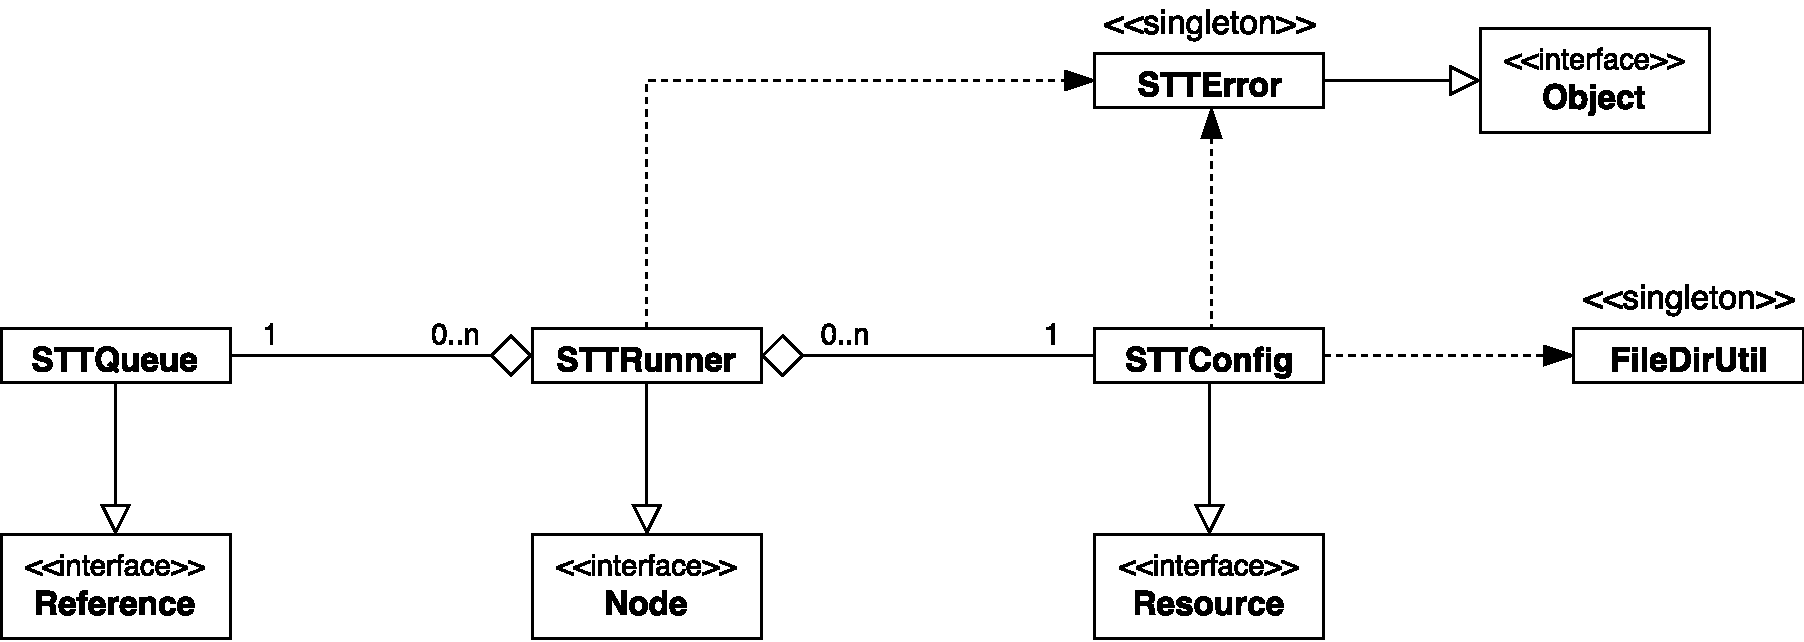
\includegraphics[width=\textwidth]{image/stt-module-simple.pdf}
  \caption{Diagrama de classes simplificado do módulo \textit{Speech to Text}}
  \label{sttModuleClassDiagram}
\end{figure}

Antes de nos aprofundarmos na arquitetura do módulo, algumas observações gerais devem ser feitas:

\begin{itemize}
\item \textit{Godot} não permite que construtores e destrutores possuam argumentos como uma forma de padronizar o instanciamento e liberação de objetos. A restrição aos construtores, no entanto, pode ser contornada através de \textit{setters} para atributos desejados.

\item A \textit{game engine} oferece implementações próprias de alguns tipos e estruturas de dados. Destacamos \texttt{String} para cadeias de caracteres e \texttt{Vector} como um vetor de uso geral, podendo representar uma fila, pilha, etc.

\item O uso de duas classes \textit{singleton} no módulo parece exagero. A justificativa é que \textit{Godot} proíbe a exportação de classes que não podem ser instanciadas (em outras palavras, classes que só possuem métodos estáticos) para uso em \mbox{\textit{GDScript}}. Recomenda-se, portanto, esta outra abordagem para contornar tal limitação \citep{godotStaticClasses}.

\item Quase todas as classes implementadas, exceto \textit{FileDirUtil}, possuem um método especial chamado \texttt{\_bind\_methods()}. Esta função, de nome predefinido por \textit{Godot}, é usada para ligar nomes a constantes ou referências de métodos, permitindo seu uso em \mbox{\textit{GDScript}}. Todas as ligações são guardadas numa grande classe \textit{singleton} denominada \textit{ObjectTypeDB}. A listagem \ref{configBindMethods} exemplifica a adição de uma linha no método \texttt{\_bind\_methods()} de \textit{STTConfig} para ser possível usar o método \texttt{init()} desta mesma classe em \mbox{\textit{GDScript}}.

\begin{lstlisting}[
  language=C++,
  label=configBindMethods,
  caption={Adicionando o método \texttt{init()} de \textit{STTConfig} para uso em \mbox{\textit{GDScript}}}
]
void STTConfig::_bind_methods() {
    ObjectTypeDB::bind_method("init", &STTConfig::init);
}
\end{lstlisting}
\end{itemize}

% ---------------------------------------------------------------------

\subsection{Classe \textit{STTConfig}}
\label{stt-config}

Como o nome sugere, \textit{STTConfig} é uma classe de configuração para a realização do reconhecimento de voz. Por possuir a característica de servir mais como um armazenamento de informação, decidimos fazer a classe herdar de \textit{Resource} (visto na seção \ref{godotResource}).

A figura \ref{stt-config-diagram} apresenta os atributos, métodos e relacionamentos da classe \textit{STTConfig}. O construtor e destrutor foram omitidos por simplicidade. Todos os atributos e métodos estáticos, neste e em futuros diagramas, estarão \underline{sublinhados}.

\begin{figure}[H]
  \centering
  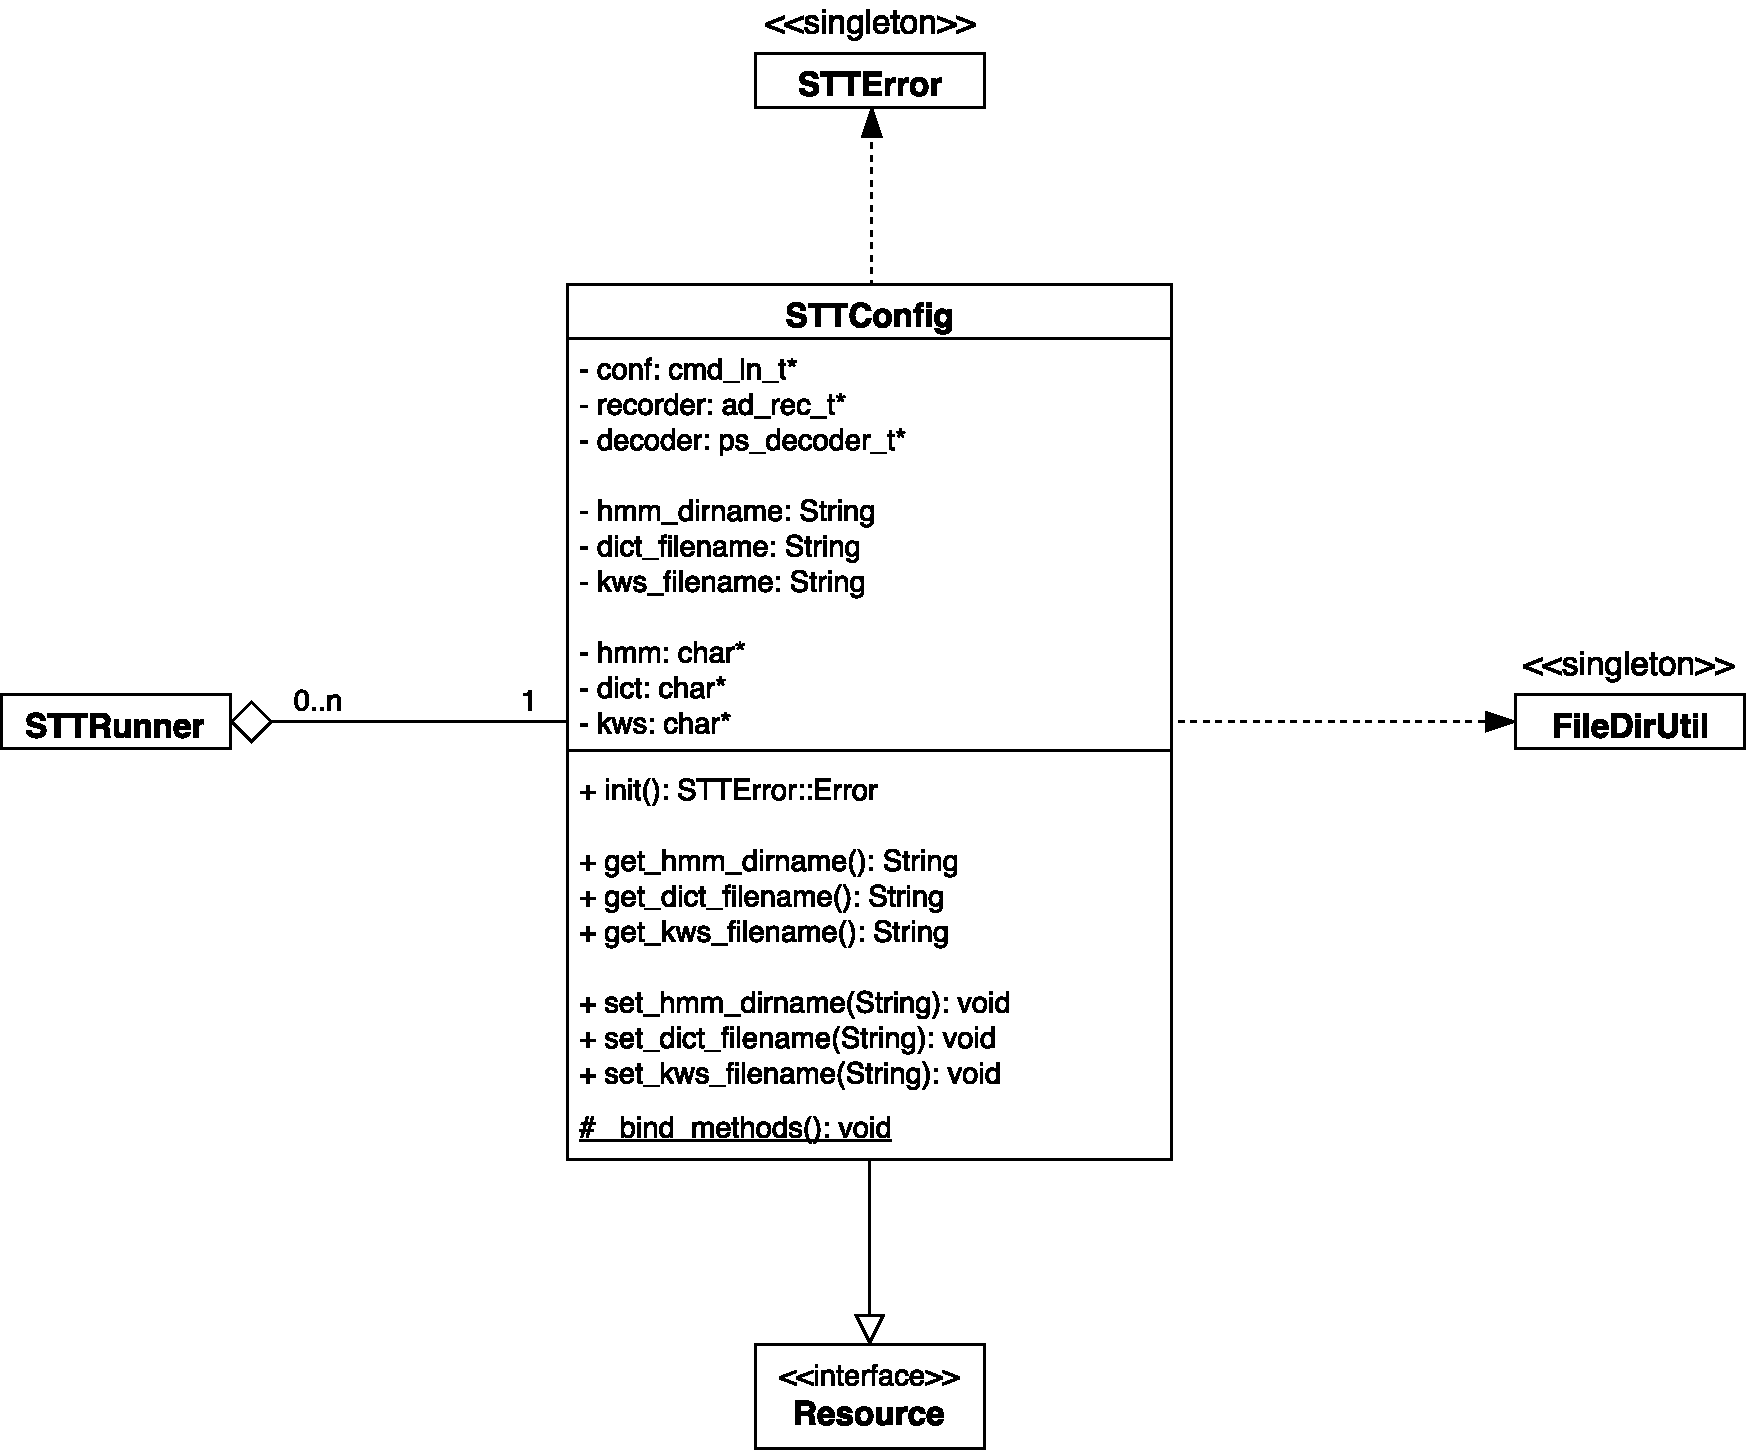
\includegraphics[width=.9\textwidth]{image/stt-config.pdf}
  \caption{Atributos, métodos e relacionamentos da classe \textit{STTConfig}}
  \label{stt-config-diagram}
\end{figure}

\textit{STTConfig} possui duas funcionalidades principais:

\subsubsection{Definir arquivos de configuração}

Nomes de arquivos de configuração são tratados pelos \textit{getters} e \textit{setters} de \texttt{hmm\_dirname}, \texttt{dict\_filename} e \texttt{kws\_filename}, que correspondem, respectivamente, ao diretório do modelo acústico, o arquivo de dicionário e o arquivo de palavras-chaves.

Verifica-se se os nomes passados como argumentos para os \textit{setters} correspondem a arquivos/diretórios existentes. No entanto, infelizmente não há como checar facilmente, em tempo de execução, se o arquivo/diretório possui erros de sintaxe. O diretório do modelo acústico, por exemplo, contém arquivos binários que, a princípio, parecem impossíveis de serem verificados. Optamos, portanto, pela filosofia de ``atirar primeiro, perguntar depois'' ao avisar posteriormente que houve problemas no uso dos arquivos.

Por fim, resta um problema para tratarmos, resultante da distinção entre os sistemas de arquivo de \textit{Godot} (visto na seção \ref{godotFileSystem}) e \textit{Pocketsphinx}. Suponha que o desenvolvedor de um jogo tenha guardado seu arquivo de dicionário, o \texttt{dicionario.dict}, na raiz do projeto. Como referenciar este arquivo? \textit{Godot} utilizaria o caminho \texttt{res://dicionario.dict}, mas \textit{Pocketsphinx} não entende este prefixo, necessitando do caminho absoluto usado no sistema.

Uma solução simples seria converter o caminho com \texttt{res://} para o caminho absoluto do sistema operacional; o método \texttt{???} da classe \textit{???} de \textit{Godot} faz justamente isso. No entanto, se o jogo estiver no formato de um binário fechado, é impossível referenciar qualquer arquivo dentro dele por meio da plataforma hospedeira.

A solução final implementada envolve usar o outro prefixo definido pela \textit{game engine}, o \textbf{\texttt{user://}}. Copiam-se todos os arquivos e diretórios de configuração para este caminho e usa-se o método \texttt{get\_data\_dir()} da classe \textit{OS} para buscar seu equivalente na plataforma hospedeira. Por precaução, adotou-se a prática de sobrescrever arquivos e diretórios copiados previamente.

\subsubsection{Inicializar variáveis do \textit{Pocketsphinx}}

A inicialização de varíaveis usadas por \textit{Pocketsphinx} é feita através de \texttt{init()}. Os nomes do diretório do modelo acústico, do arquivo de dicionário e do arquivo de palavras-chave precisam ter sido definidos previamente com os apropriados \textit{setters}, ou o método retornará um número de erro.

Deparamo-nos com outro problema de compatibilidade: os nomes dos arquivos são fornecidos com o tipo \texttt{String} adotado por \textit{Godot}. No entanto, \textit{Pocketsphinx} não conhece este tipo, utilizando o \texttt{char *} comumente encontrado em \textit{C} para receber estes mesmos nomes. Felizmente, \texttt{String} possui um método \texttt{c\_str()} para realizar a conversão.

% TODO: Fix reference below

O método \texttt{init()} irá inicializar as variáveis de configuração \texttt{cmd\_ln\_t}, de gravação de voz \texttt{ad\_rec\_t} e o decodificador \texttt{ps\_decoder\_t} (todos vistos na seção \ref{???}). Caso algum problema ocorra, retorna-se um número de erro, pertencente à classe \mbox{\textit{STTError}}, relativo ao problema ocorrido.

A cópia de arquivos para o caminho \textit{user://}, mencionada anteriormente, também ocorre neste método.

% ---------------------------------------------------------------------

\subsection{Classe \textit{STTRunner}}

\textit{STTRunner} é a classe responsável por realizar o reconhecimento de voz em si. Por claramente implementar uma \textbf{funcionalidade} a ser usada pelo usuário do editor \textit{Godot}, decidiu-se que uma herança de \textit{Node} (visto na seção \ref{godotNode}) seria bastante apropriada.

A figura \ref{stt-runner-diagram} apresenta os atributos, métodos e relacionamentos da classe \textit{STTRunner}. O construtor e destrutor foram omitidos por simplicidade.

\begin{figure}[H]
  \centering
  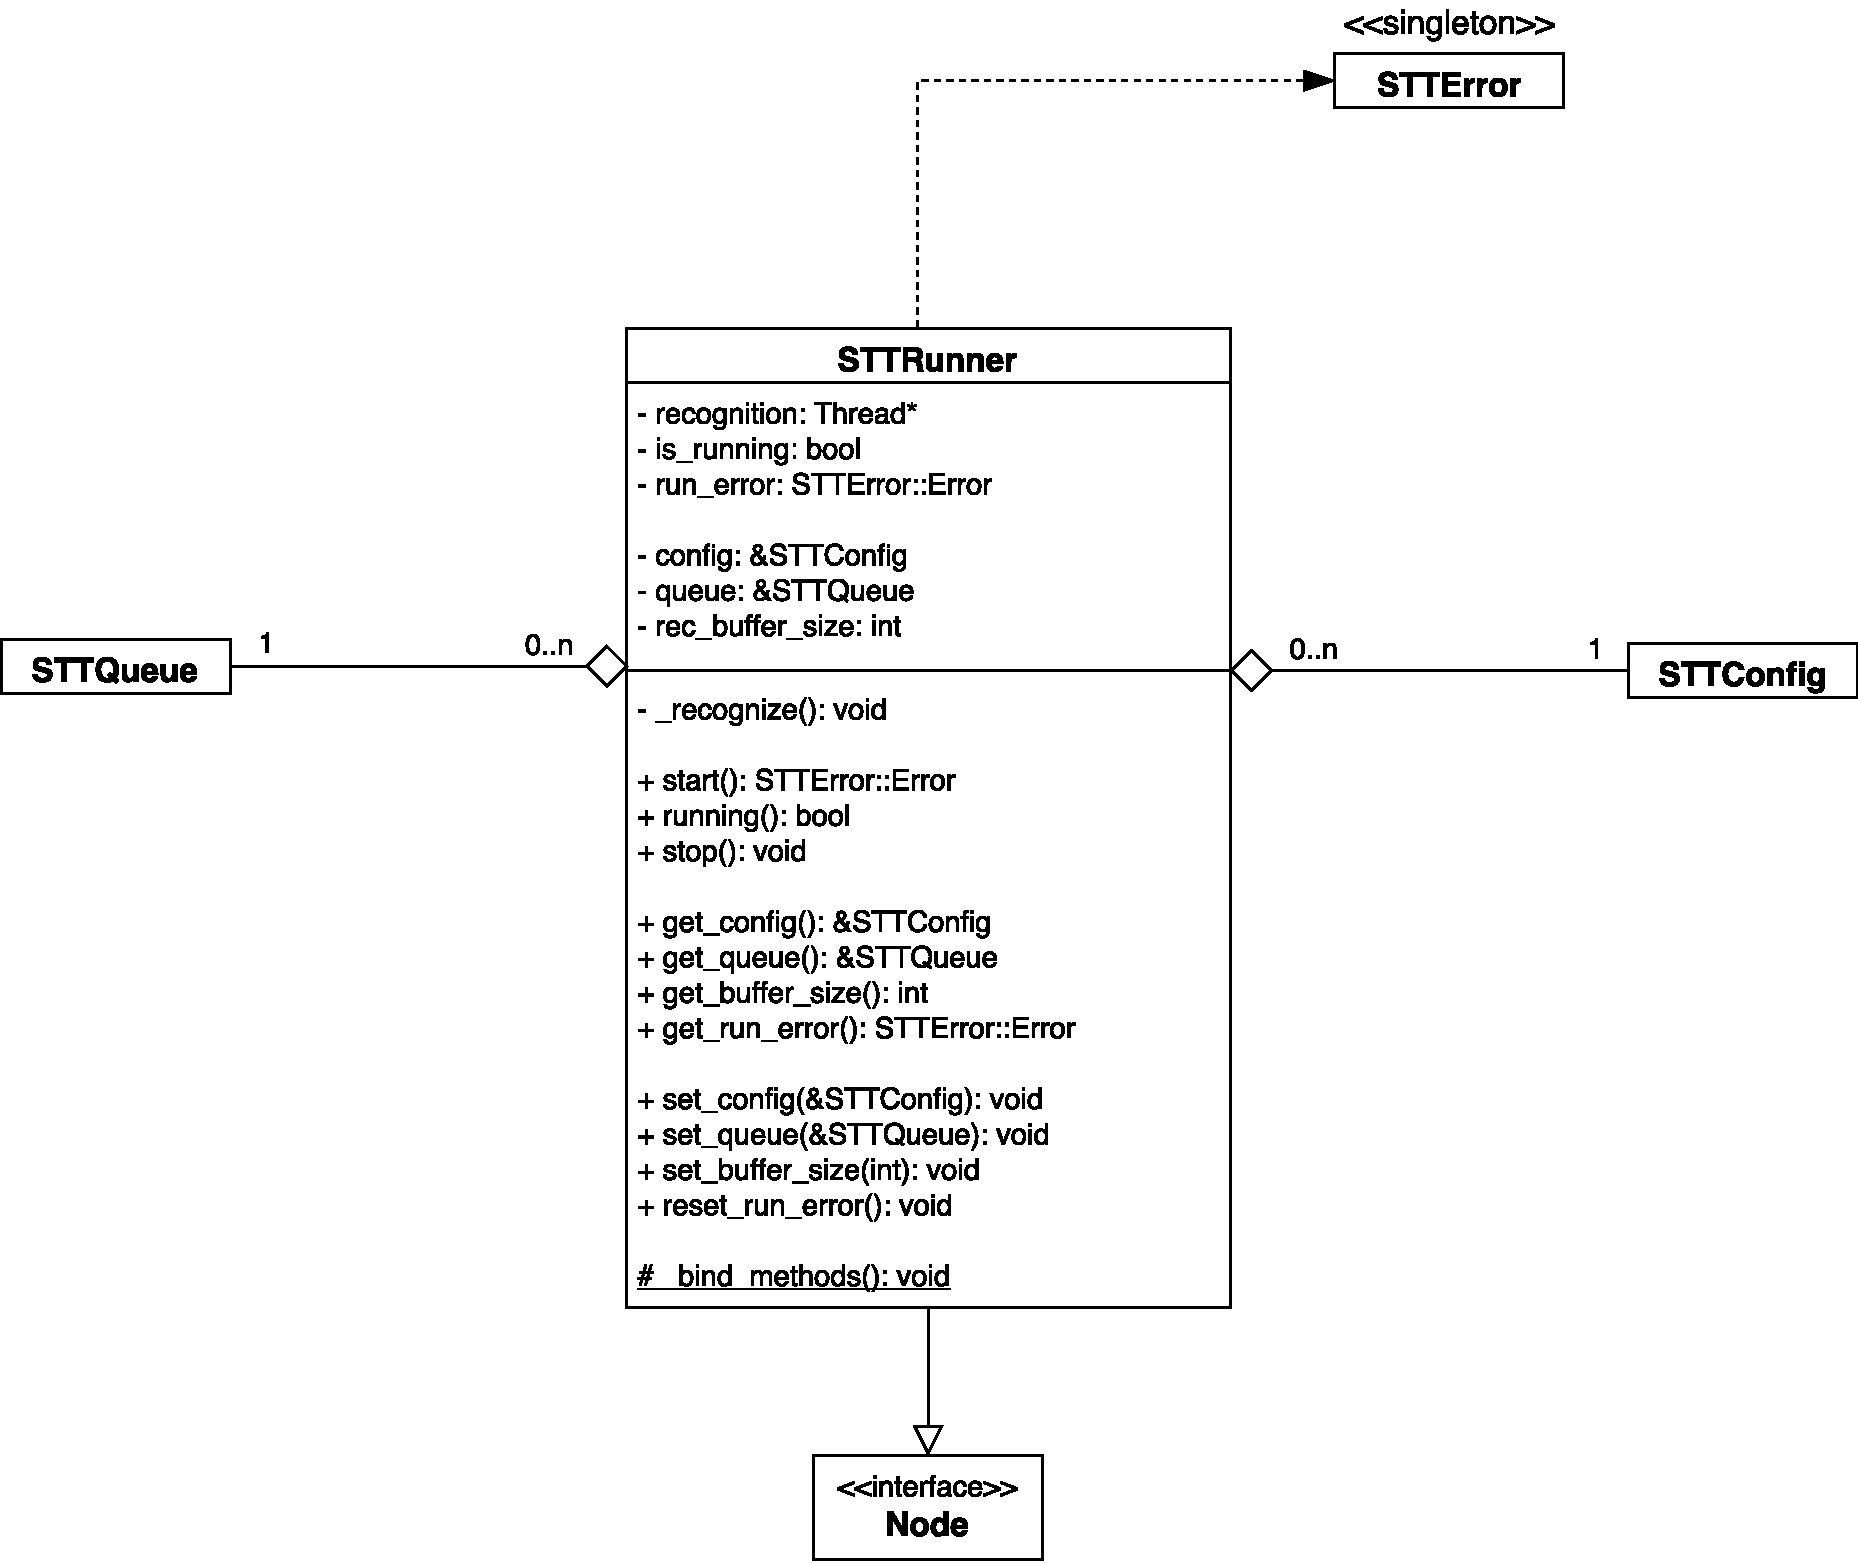
\includegraphics[width=.9\textwidth]{image/stt-runner.pdf}
  \caption{Atributos, métodos e relacionamentos da classe \textit{STTRunner}}
  \label{stt-runner-diagram}
\end{figure}

A classe usa um objeto \textit{STTConfig} para obter as variáveis \textit{Pocketsphinx} necessárias em sua tarefa, e um objeto \textit{STTQueue} para guardar termos (palavras ou pequenas frases) gerados no reconhecimento de voz. Ambos podem ser obtidos e definidos através dos \textit{getters} e \textit{setters} para \texttt{config} e \texttt{queue}.

Comentamos, nos requisitos funcionais (seção \ref{moduleFunctionalRequirements}), que o reconhecimento deveria ocorrer em paralelo com o restante do jogo. O uso de uma \textit{thread} serve bem para tal propósito; \textit{Godot}, inclusive, oferece uma implementação própria dessa estrutura em sua classe \textit{Thread}. Os dois métodos mais importantes que usaremos dela são:

\begin{itemize}
\item \texttt{Thread * create(função, argumento, configurações)}: Cria uma \textit{thread} para executar uma função \texttt{f(void *arg)}. O parâmetro \textit{função} corresponde ao nome de \texttt{f} e \textit{argumento}, a \texttt{arg}. Opcionalmente, podem ser passadas configurações adicionais como um terceiro parâmetro, mas não entraremos em detalhes por não terem sido necessárias. Retorna-se um ponteiro para a instância de \textit{Thread} criada.

\item \texttt{void wait\_to\_finish(thread)}: Recebe um ponteiro para uma instância de \textit{Thread}. Espera a \textit{thread} terminar, finalizando-a com segurança.
\end{itemize}

O método \texttt{start()} cria uma \textit{thread} para realizar o reconhecimento de voz desde que o objeto \textit{STTRunner} já possua instâncias de \textit{STTConfig} e \textit{STTQueue}. Chama-se \texttt{Thread::create()} com um método estático como parâmetro (\texttt{\_thread\_recognize()}, que não aparece na figura \ref{stt-runner-diagram} por agir apenas como um intermédio) e a própria instância como argumento (isto é, \texttt{this}).

A listagem \ref{thread-recognize} mostra a implementação de \texttt{\_thread\_recognize()}, responsável por chamar o método privado \texttt{\_recognize()} da instância passada como argumento. É nesta última função que o laço de reconhecimento de voz ocorre, implementado de forma bastante similar ao que vimos na seção \ref{???}.

\begin{lstlisting}[
  language=C++,
  label=thread-recognize,
  caption={Método estático \texttt{\_thread\_recognize()} de \textit{STTRunner}}]
void STTRunner::_thread_recognize(void *runner) {
    STTRunner *self = (STTRunner *) runner;
    self->_recognize();
}
\end{lstlisting}

Para controle sobre a \textit{thread}, o usuário do módulo pode verificar sua execução com \texttt{running()} e ordenar sua parada imediata com \texttt{stop()}. Definiu-se que apenas uma \textit{thread} pode existir por instância de \textit{STTRunner}, pois o controle de várias operações em paralelo não traria nenhum benefício ao módulo.

Por fim, oferece-se controle sobre o tamanho do \textit{buffer} de gravação de voz através do \textit{getter} e \textit{setter} de \texttt{buffer\_size}. É importante ressaltar que o uso de um \textit{setter} demanda a parada imediata da \textit{thread} de reconhecimento para evitar possíveis problemas de acesso antes e depois da alteração (condição de corrida).

% ---------------------------------------------------------------------

\subsection{Classe \textit{STTQueue}}

\textit{STTQueue} implementa um \textit{buffer} para guardar palavras geradas no reconhecimento de voz, conforme planejado nos requisitos funcionais (seção \ref{moduleFunctionalRequirements}). Fizemos que com herdasse da classe \textit{Reference} (visto na seção \ref{godotReference}) com o intuito de simplificar seu gerenciamento de memória.

É usado por \textit{STTRunner} para guardar termos do reconhecimento de voz. Ao mesmo tempo, o usuário do módulo pode retirar estes termos do módulo e usá-los no jogo.

A figura \ref{stt-queue-diagram} apresenta os atributos, métodos e relacionamentos da classe \textit{STTQueue}. O construtor e destrutor foram omitidos por simplicidade.

\begin{figure}[H]
  \centering
  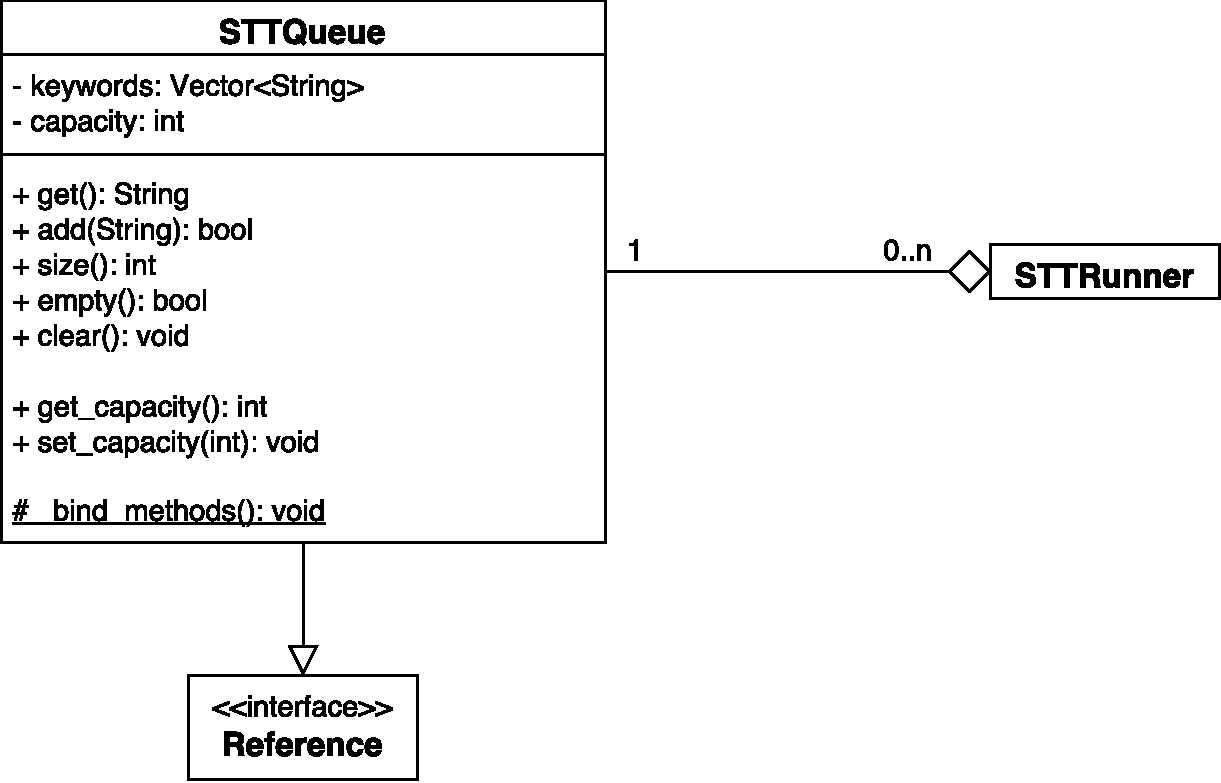
\includegraphics[width=.8\textwidth]{image/stt-queue.pdf}
  \caption{Atributos, métodos e relacionamentos da classe \textit{STTQueue}}
  \label{stt-queue-diagram}
\end{figure}

Conforme o nome sugere, o tipo abstrato de dados usado para o \textit{buffer} da \textit{STTQueue} é uma \textbf{fila}. \textit{Godot} implementa esta estrutura, com diversas funcionalidade a mais, em sua classe \textit{Vector}. Como muitas de seus métodos seriam desnecessários (não é necessário, por exemplo, que o usuário possa ordenar a fila de reconhecimento de voz), \textit{STTQueue} age como um intermédio do que pode e não pode ser feito em \textit{Vector}.

Os principais métodos de \textit{STTQueue} estão resumidos na tabela \ref{stt-queue-main-methods}.

\begin{table}[H]
\centering

\begin{tabular}{|c|l|}
\hline
\textbf{Método}  & \thead{\textbf{Descrição}}                          \\ \hline
\texttt{get()}   & Retira e retorna a primeira \texttt{String} da fila \\ \hline
\texttt{add()}   & Adiciona uma \texttt{String} no final da fila       \\ \hline
\texttt{size()}  & Retorna o número de elementos atualmente na fila    \\ \hline
\texttt{empty()} & Retorna \texttt{true} se a fila estiver vazia       \\ \hline
\texttt{clear()} & Esvazia a fila, removendo todos os seus elementos   \\ \hline
\end{tabular}

\caption{Principais métodos de \textit{STTQueue}}
\label{stt-queue-main-methods}
\end{table}

O leitor pode se perguntar se não ocorre condição de corrida no acesso à fila: há risco de se perder algum dado quando \textit{STTRunner} realiza um \texttt{add()} ao mesmo tempo em que o usuário utiliza \texttt{get()}, por exemplo? Felizmente, a implementação de \texttt{Vector} é \textit{thread-safe}, garantindo que esses problemas não ocorram.

Uma decisão deveria ser tomada quanto a um caso particular de \texttt{get()}: o que fazer quando o método fosse chamado com uma fila vazia? Nesta situação, decidiu-se retornar uma \texttt{String} vazia (\texttt{``''}) e simultaneamente imprimir uma mensagem de \textit{warning} devido ao uso impróprio. Recomenda-se, portanto, verificar o tamanho da fila com \texttt{empty()} antes do uso de \texttt{get()}.

Além dos métodos da tabela \ref{stt-queue-main-methods}, há mais dois que foram criados para definir um limite superior para o número de elementos na fila. Este valor pode ser lido e alterado por \texttt{get\_capacity()} e \texttt{set\_capacity()}, respectivamente. O usuário, teoricamente, não deveria permitir um acúmulo muito grande de palavras na fila, mas se tal caso ocorrer, ao menos o consumo de memória fica controlado.

% ---------------------------------------------------------------------

\subsection{Classe \textit{STTError}}

\textit{STTError} define constantes numéricas para possíveis erros que podem ocorrer no módulo (mais especificamente, em \textit{STTConfig} e \textit{STTRunner}). A utilidade da classe, portanto, está em ajudar o usuário a entender melhor a causa de um erro que possa vir a ocorrer no módulo. Por ser um \textit{singleton} mas ter seu uso necessário no editor \textit{Godot} (através de \mbox{\textit{GDScript}}), decidiu-se fazer a classse herdar de \textit{Object} (visto na seção \ref{godotObject}).

A figura \ref{stt-error-diagram} apresenta os atributos, métodos e relacionamentos da classe \textit{STTError}. O construtor e destrutor foram omitidos por simplicidade.

\begin{figure}[H]
  \centering
  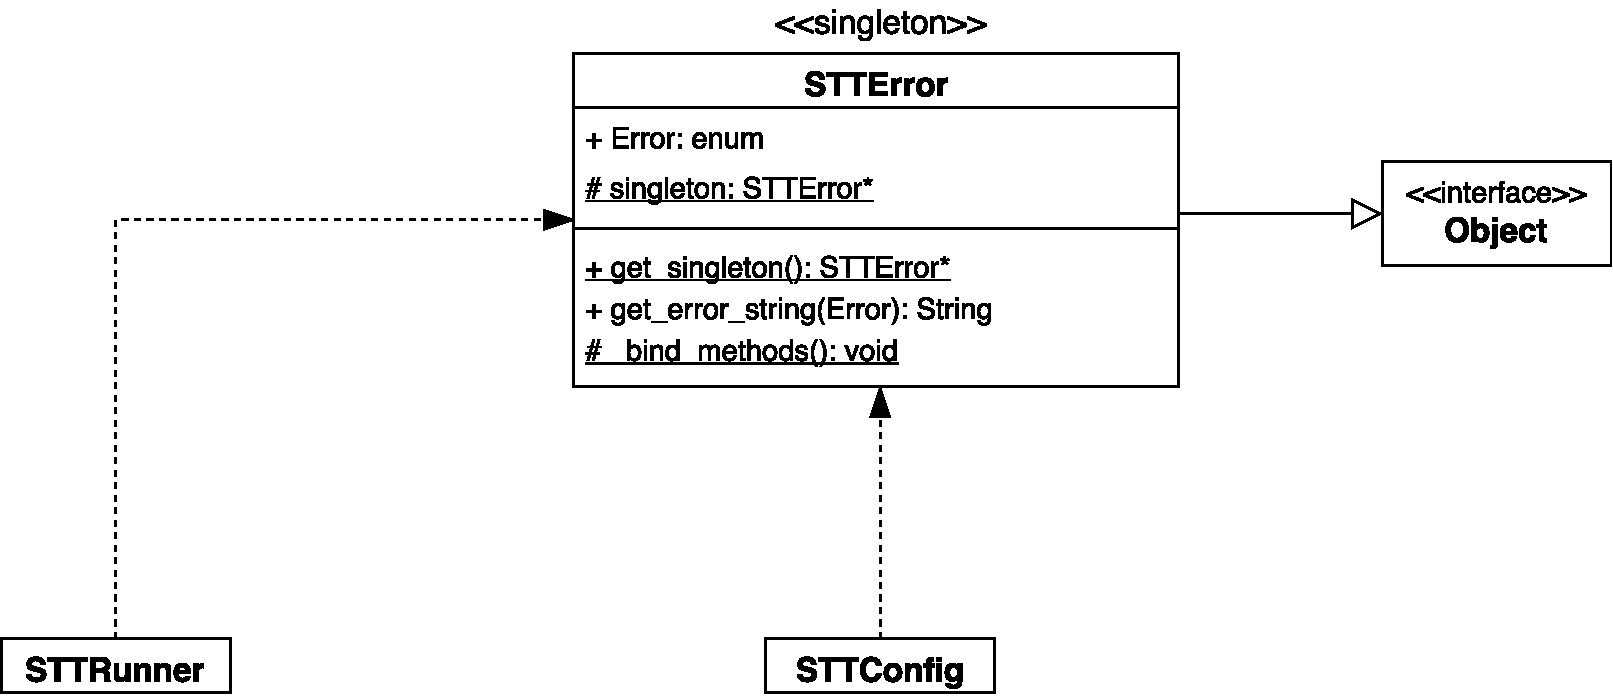
\includegraphics[width=.9\textwidth]{image/stt-error.pdf}
  \caption{Atributos, métodos e relacionamentos da classe \textit{STTError}}
  \label{stt-error-diagram}
\end{figure}

Alguns métodos de \textit{STTConfig} e \textit{STTRunner} retornam um número definido pelo \texttt{enum Error}. Uma \texttt{String} contendo a interpretação deste valor pode ser obtida chamando-se o método \texttt{get\_error\_string()} da classe.

A tabela \ref{stt-error-enum} contém os valores definidos no \texttt{enum Error}, bem como suas respectivas interpretações.

\begin{table}[H]
\centering

\begin{tabularx}{\linewidth}{|l|X|}
\hline
\thead{\textbf{Erro}} & \thead{\textbf{Interpretação}} \\ \hline
\texttt{OK} & Nenhum erro ocorreu \\ \hline
\texttt{UNDEF\_FILES\_ERR} & Um ou mais nomes de arquivos/diretórios de configuração não foram definidos \\ \hline
\texttt{UNDEF\_CONFIG\_ERR} & Um objeto \texttt{STTConfig} não foi definido \\ \hline
\texttt{UNDER\_QUEUE\_ERR} & Um objeto \texttt{STTQueue} não foi definido \\ \hline
\texttt{USER\_DIR\_MAKE\_ERR} & Erro ao criar o diretório STT em \texttt{user://} \\ \hline
\texttt{USER\_DIR\_COPY\_ERR} & Erro ao copiar arquivos de configuração para \texttt{user://} \\ \hline
\texttt{MULTIBYTE\_STR\_ERR} & Erro ao converter o nome do arquivo para uma sequência de vários bytes \\ \hline
\texttt{MEM\_ALLOC\_ERR} & Não há memória disponível para alocação \\ \hline
\texttt{CONFIG\_CREATE\_ERR} & Erro criar a variável de configuração de \textit{Pocketsphinx} \\ \hline
\texttt{REC\_CREATE\_ERR} & Erro ao se conectar o aparelho de áudio (microfone) \\ \hline
\texttt{DECODER\_CREATE\_ERR} & Erro ao criar a variável de decodificação de \textit{Sphinxbase} \\ \hline
\texttt{REC\_START\_ERR} & Erro ao começar a gravar a voz do usuário \\ \hline
\texttt{REC\_STOP\_ERR} & Não foi possível parar a gravação da voz do usuário \\ \hline
\texttt{UTT\_START\_ERR} & Erro ao iniciar a captura de \textit{utterance} durante o reconhecimento de voz \\ \hline
\texttt{UTT\_RESTART\_ERR} & Erro ao reiniciar a captura de \textit{utterance} durante o reconhecimento de voz \\ \hline
\texttt{AUDIO\_READ\_ERR} & Erro ao ler dados da gravação de áudio \\ \hline
\end{tabularx}

\caption{Valores de erro definidos em \texttt{enum Error} e suas interpretações}
\label{stt-error-enum}
\end{table}

% ---------------------------------------------------------------------

\subsection{Classe \textit{FileDirUtil}}

\textit{FileDirUtil} é uma classe auxiliar, não possuindo relação alguma com reconhecimento de voz. Como o nome sugere, ela possui métodos para manipular arquivos e diretórios.

A figura \ref{file-dir-util-diagram} apresenta os métodos e relacionamento da classe \textit{FileDirUtil}. O construtor e destrutor foram omitidos por simplicidade.

\begin{figure}[H]
  \centering
  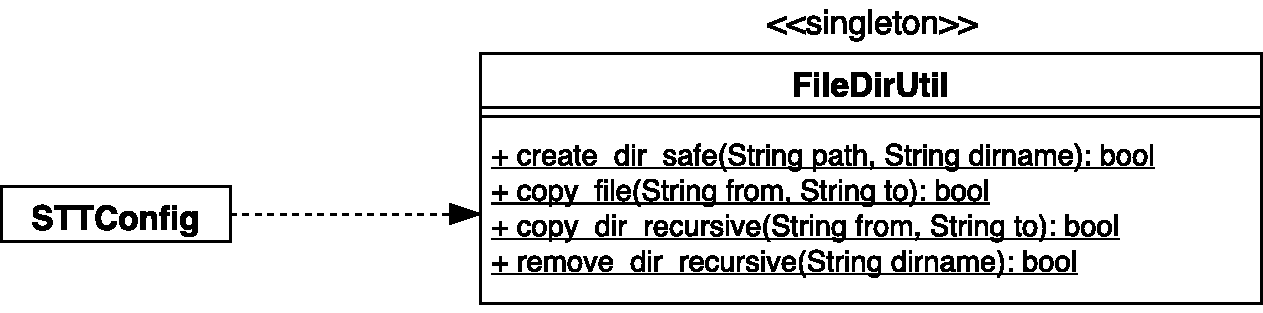
\includegraphics[width=.75\textwidth]{image/file-dir-util.pdf}
  \caption{Atributos, métodos e relacionamentos da classe \textit{FileDirUtil}}
  \label{file-dir-util-diagram}
\end{figure}

As ferramentas oferecidas por \textit{Godot} para gerenciamento de arquivos e diretórios são bem simples, limitando-se ao seguinte: criação de arquivos/diretórios, escrita/leitura/cópia de arquivos, remoção de arquivos individuais e diretórios vazios.

Vimos que \textit{STTConfig} necessita copiar os arquivos de configuração para \texttt{user://}. \textit{FileDirUtil} meramente combina os métodos já implementados pela \textit{game engine} para realizar operações como cópia e remoção recursiva de diretórios.

% ---------------------------------------------------------------------

\section{Arquivos e \textit{scripts} de configuração}

% ---------------------------------------------------------------------

\subsection{\texttt{register\_types}}

% ---------------------------------------------------------------------

\subsection{\texttt{SCsub}}

% ---------------------------------------------------------------------

\subsection{\texttt{config.py}}

% ---------------------------------------------------------------------

\section{Divulgação}

Todo o código fonte do módulo \textit{Speech to Text} encontra-se em um repositório no GitHub do autor \citep{sttModuleGitHub}, juntamente com instruções para compilação e uso. Também foram disponibilizados binários dos editores \textit{Godot} e \textit{templates de exportação}, ambos compilados previamente com o módulo \citep{sttModuleDownload}.

\textit{Speech to Text} foi divulgado em dois fóruns de \textit{Godot}, onde obteve algumas poucas aprovações:

\begin{itemize}
\item \textbf{Godot Engine Q\&A} \citep{sttModuleGodotQA}: O site oficial de \textit{Godot} disponibiliza uma seção para perguntas e respostas, onde existe uma subseção para publicação de projetos.

\item \textbf{Godot Developers} \citep{sttModuleGodotDevelopers}: Embora seja mais voltado para jogos produzidos na \textit{game engine}, este fórum possui uma seção para compartilhamento de recursos e ferramentas.
\end{itemize}
